\chapter{Functioneel Ontwerp}\label{ch:functioneel-ontwerp} % Chapter title

%TODO: MarginPARS zetten
\label{funtioneelOntwerp} % For referencing the chapter elsewhere, use \autoref{ch:InOnderzoek}

Na het inzicht dat verkregen is na het onderzoek zijn er de volgende requirements bij gekomen.
De volledige lijst zal vervolgens worden gebruikt om een functioneel ontwerp te maken.


\section{Architectuur ontwerp}\label{sec:architectuur-ontwerp}
Uit de requirements blijkt dat de module moet samenwerken met een aantal systemen binnen EagleScience. in figuur~\ref{fig:UML-ComponentDiagram} is te zien dat de SOUP-API een centraal onderdeel is van de module. Het is verantwoordelijk voor verschillende taken die nodig zijn voor de informatie behoefte die de module moet weergeven.

\begin{figure}[bth]
    \myfloatalign
    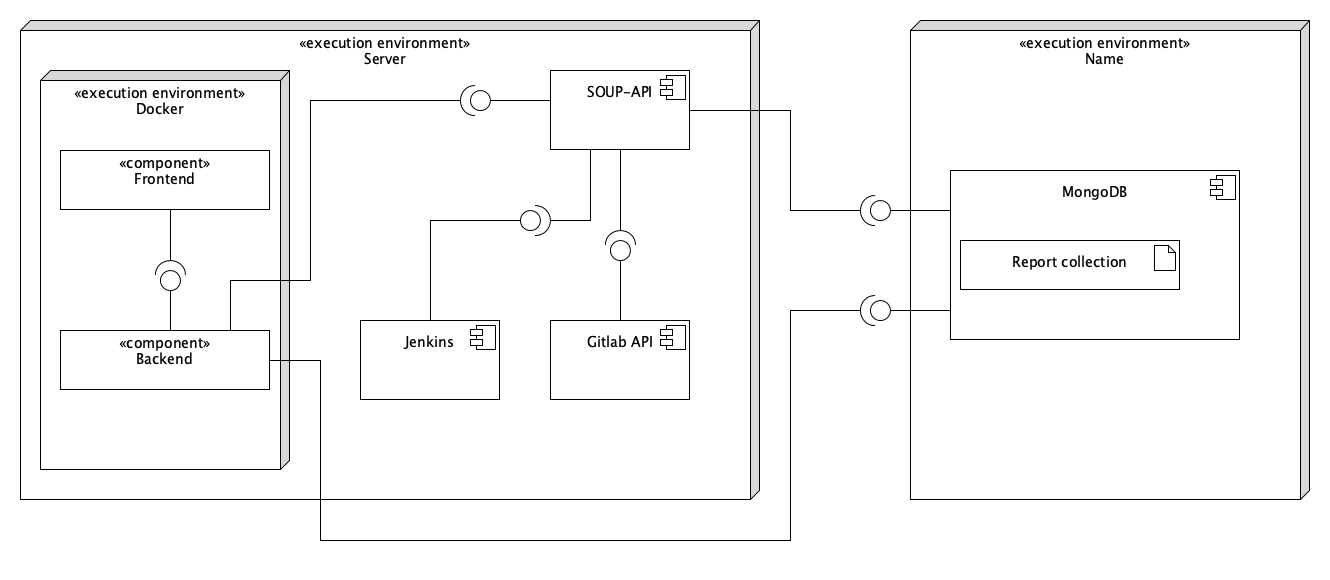
\includegraphics[width=15cm]{gfx/UMLcomponent diagram}
    \caption{Component diagram}
    \label{fig:UML-ComponentDiagram}
\end{figure}

\section{SOUP-API}\label{sec:soup-api}
Er \textbg{\textit{MOET}} nog een betere naam worden verzonnen.
DE SOUP-API is het centrale onderdeel van de module. Het heeft de functie rapporten te genereren. De generatie moet op twee momenten worden gedaan. Ten eerste als er nieuwe code in wordt gecheckt in Jenkins en ten tweede als een project al een tijd op productie draait moet er periodiek worden gecontroleerd of de gebruikte bibliotheken nog up-to-date en vooral veilig zijn.

\subsection{process: periodiek Checken van een repository op basis van nieuwe }\label{subsec:process:-periodiek-checken}
Er is een process nodig om periodiek een raport te genereren die inzicht geeft in de huidige staat van kwetbaarheden voor projecten.

\begin{enumerate}
    \item User doet POST request op "\textbackslash createreport?project="PROJECTNAAM"
    \item 
\end{enumerate}


